\documentclass[letterpaper, 12pt]{math}

\usepackage{tikz}
\usetikzlibrary{backgrounds}
\usetikzlibrary{decorations.pathmorphing,patterns}

\title{University Physics 1A}
\author{Alvin Lin}
\date{October 12th, 2017}

\begin{document}

\maketitle

\section*{Conservation of Energy}
A ball of mass \( m \) is launched from a vertical spring of spring
constant \( k \). It reaches its maximum height above the equilibrium
position of the spring in a time \( t \) after launch. Say you are asked to
find the initial compression of the spring relative to equilibrium in terms
of the variables provided and \( g \). Note that the maximum height is not a
provided value.
\begin{center}
  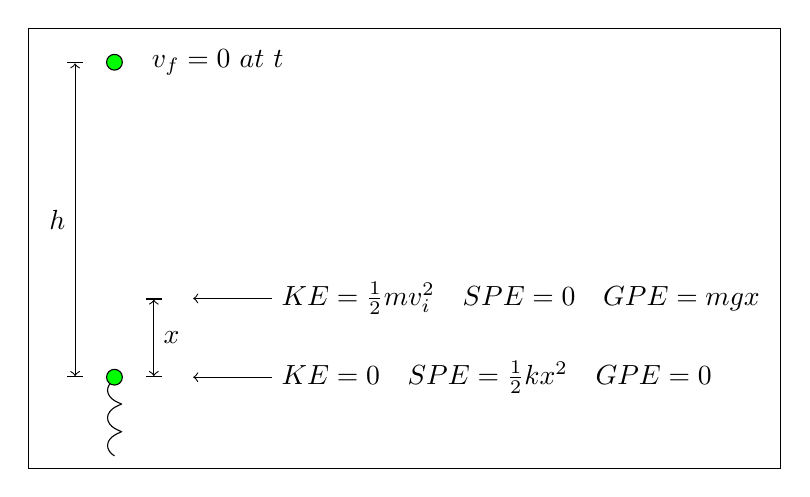
\begin{tikzpicture}[framed]
    \draw[decoration={coil},decorate] (0,0) -- (0,1);
    \draw[fill=green] (0,1) circle (0.1cm);
    \draw[fill=green] (0,5) circle (0.1cm) node[right]
      {\(\quad v_f = 0~at~t \)};
    \draw[|<->|] (0.5,1) -- (0.5,2) node[pos=0.5, right] {\( x \)};
    \draw[|<->|] (-0.5,1) -- (-0.5,5) node[pos=0.5, left] {\( h \)};
    \draw[<-] (1,1) -- (2,1) node[pos=1, right]
      {\( KE = 0\quad SPE = \frac{1}{2}kx^2\quad GPE = 0 \)};
    \draw[<-] (1,2) -- (2,2) node[pos=1, right]
      {\( KE = \frac{1}{2}mv_i^2\quad SPE = 0\quad GPE = mgx \)};
  \end{tikzpicture}
\end{center}
\begin{align*}
  0 &= v_f = v_i+at \\
  v_i &= -at \\
  \frac{1}{2}kx^2 &= \frac{1}{2}mv_i^2+mgx \\
  0 &= \frac{1}{2}kx^2-mgx-\frac{1}{2}m(-at)^2
\end{align*}
\begin{align*}
  0 &= \left(\frac{1}{2}k\right)x^2+(-mg)x-\frac{1}{2}ma^2t^2 \\
  a &= \frac{1}{2}k \\
  b &= -mg \\
  c &= -\frac{1}{2}ma^2t^2 \\
  x &= \frac{-b\pm\sqrt{b^2-4ac}}{2a} \\
  &= \frac{-mg\pm\sqrt{(mg)^2+kma^2t^2}}{k}
\end{align*}

In a new exciting ride, a roller-coaster car passed the top of one hill, then
rolls to the bottom on a track. It then heads up a flat ramp and flies off the
end of the ramp. Suppose that the car has a speed of 0.9m/s at the top of the
hill, which is 8.0m off the ground. Say the ramp has a height of 1.0m above the
ground and makes an angle of \( 30.0^{\circ} \) with the horizontal. Model
this problem so that air resistance and friction are negligible. Use ideas of
energy and kinematics to find the following:
\begin{enumerate}
  \item the speed of the car as it leaves the ramp.
  \begin{align*}
    KE_i+PE_i &= KE_f+PE_f \\
    \frac{1}{2}mv_i^2+mgh_i &= \frac{1}{2}mv_f^2+mgh_f \\
    \frac{1}{2}(9^2)+g(8) &= \frac{1}{2}v_f^2+g(1) \\
    v_f &= 14.77\frac{m}{s}
  \end{align*}
  \item the speed of the car when it reaches maximum height in the air after
  leaving the ramp.
  \begin{align*}
    v_y &= 0 \\
    v_x &= v\cos\theta \\
    &= 14.77\cos(30) \\
    &= 12.79\frac{m}{s}
  \end{align*}
  \item the maximum height that the car reaches above the ground after leaving
  the ramp.
  \begin{align*}
    v_f^2 &= v_i^2+2gd \\
    0 &= (14.8\sin(30))^2+2(-9.8)d \\
    d &= 2.8m \\
    d+x_0 &= 2.8+1 = 3.8m
  \end{align*}
\end{enumerate}

\begin{center}
  You can find all my notes at \url{http://omgimanerd.tech/notes}. If you have
  any questions, comments, or concerns, please contact me at
  alvin@omgimanerd.tech
\end{center}

\end{document}
